\section{Introduction}
Given a non-empty set $\mathcal{A}$, a partition $\Pi$ of $\mathcal{A}$ is defined as a collection of subsets of $\mathcal{A}$, i.e., $\Pi = \{A_1, A_2, \ldots, A_k\}$, such that:

\begin{itemize}
    \item $\bigcup\limits_{i = 1}^{k} A_i = \mathcal{A}$.
    \item $A_i \cap A_j = \emptyset$ for all $i \neq j$.
\end{itemize}

The elements of $\Pi$ are called \textit{classes}. Furthermore, we define an equivalence relation between two elements $a, b \in \mathcal{A}$ by stating that $a$ and $b$ are equivalent if and only if there exists some $A_i \in \Pi$ such that $a, b \in A_i$. In this case, we say that $a$ and $b$ are equivalent and denote this by $a \equiv b$.

One can trivially verify that this binary relation is reflexive, symmetric, and transitive. These properties allow us to define a \textit{representative} for each class—an element that represents the entire class. By the reflexive, symmetric, and transitive properties, every other element in the same class is related to this \textit{representative}.

This concept, previously established by mathematicians, is widely used in Computer Science to implement the Union-Find data structure. The Union-Find data structure is designed to efficiently store and manage a partition of a set $\mathcal{A}$. It provides two fundamental operations:

\begin{itemize}
    \item \texttt{Find Operation:} Given an element $a \in \mathcal{A}$ find the representative of the class from which $a$ belongs.
    \item \texttt{Union Operation:} Given two element $a \in A_i$ and $b \in A_j$ make a union of classes $A_i$ and $A_j$. That is, given a partition $\Pi$ the result of the union operation will be a new partition $\Pi'$ such that $\Pi' =  (\Pi \setminus \{A_i,A_j\}) \cup (\{A_i \cup A_j\})$
\end{itemize}

\section{Implementation}
A C++ implementation has been made for the sake of efficiency of the Union-Find operations. A C++ class has been created for the Union-Find data structure (look at \texttt{UnionFind.hh} for a more detailed exploration of the class). It consists mainly of an array in which every element will either point to another element that belongs to the same class or it will be the representative. For the representative, depending on the union strategy they will be represented differently:

\begin{itemize}
    \item With the Quick-Union strategy an element $i$ is the representative of a class if $v[i] = i$.
    \item With the other strategies (union by rank/size) they will be represented by a negative number that indicates the size/rank multiplied by $-1$ (i.e. $v[i] = -size$ or $v[i] = -rank$).
\end{itemize}

The \texttt{main.cc} file requires, as input, the size of the data structure, a Union strategy (a natural number between 0 and 2, representing Quick-Union, Union by Weight, and Union by Rank, respectively), and a Path strategy (a natural number between 0 and 3, representing No Compression, Full Compression, Path Splitting, and Path Halving). After that, the program will repeatedly request two natural numbers (the elements to be merged) and perform the corresponding union operation. This process continues until the data structure consists of a single block, at which point the program terminates.

Every $\Delta = 250$ elements, the program will output information about the current TPL and TPU of the data structure. The TPU parameter is computed using a counter that increments by one each time a pointer switch occurs (see Appendix \ref{ap:Path}), while the TPL is calculated by traversing the entire data structure (see Appendix \ref{ap:TPL}). Although this approach may not be the most efficient in terms of performance, the author chose this method for computing the TPL because the focus is on obtaining the value rather than optimizing execution time. Later, execution time will be measured separately, excluding this part of the computation.

To execute the program, one can compile it using the provided \texttt{Makefile} by running \texttt{make main} and then executing the program from the command line. For instance, suppose \texttt{file.txt} contains pairs of numbers (between 0 and 999) that, when processed, will lead to a single block in the Union-Find data structure. In that case, we can process these numbers using Union by Weight and Path Halving by executing the following command:

\texttt{./main.exe 1000 1 3 < file.txt}

For getting time results you just need to compile by running \texttt{make main\_time}.

\section{Experimental Setup}
To generate random instances, a number \( n \) of elements and a seed \( s \) are requested as input. Then, this program generates a random number of different pairs \( (i, j) \) where \( 0 \leq i < j < n \) until the total number of pairs generated forms a single block in a Union-Find data structure. 

The time complexity of this program is difficult to calculate, as there is no guarantee that the program will terminate. Since it generates pseudo-random different pairs, it might enter a loop where all the pairs generated are repetitions. However, this approach is better than the initial implementation, which involved generating all possible \(n \choose 2 \) pairs—requiring \( \Theta(n^2) \) time and space complexity—and then selecting random pairs until a single block is formed in the Union-Find structure. Using this new approach we use a C++ set to keep track of all different pairs, requesting only necessary memory.

For the following experiments, $20$ instances of size ($n = 1000, 5000, 10000$) have been created. Each instance was generated with a seed $s$ that goes from $1964$ (in honor of Union-Find data structure discover\cite{galler1964improved}!) to $1983$. Each instance has been executed with the $12$ possible different strategies and the data has been collected as follows:

\begin{enumerate}
    \item For each size \( n \), union strategy and path strategy, execute all instances of size \( n \).
    \item For every instance with the same size, union strategy, and path strategy, we will average all values obtained for every \( k \in \{\Delta, 2\Delta, 3\Delta, \ldots\} \) pairs processed, as long as at least five instances have reached the point of processing \( k \) pairs.
\end{enumerate}

Although this process might be tedious, it can be automated by executing a single script! (See README).

Using these samples we gained samples for, approximately: $3750$ pairs of elements for $n = 1000$, $26250$ pairs of elements for $n = 5000$ and $52250$ pairs of elements for $n = 10000$. 

\section{Results}
\subsection{Metric Comparisons}
\subsubsection{Path Strategy: No Compression}
Using this technique, the minimization of paths between an element $i$ and its representative $r_i$ relies solely on the Union heuristic. Specifically, in the case of Quick-Union, Figure \ref{fig:tplNC} shows that Quick-Union differs significantly from TPL compared to the other union techniques. This difference makes sense, as we do not use any heuristic to help minimize those paths. 

Still we need to take a look on the performance of Union by size and Union by Weight, Figure \ref{fig:tplNC} also provides a look to such performance. As we see, there is not a big difference (although union by size performs slightly better) between these strategies in this context.

\begin{figure}[ht]
    \centering
    % Subfigure 1
    \begin{subfigure}{0.32\textwidth}
        \centering
        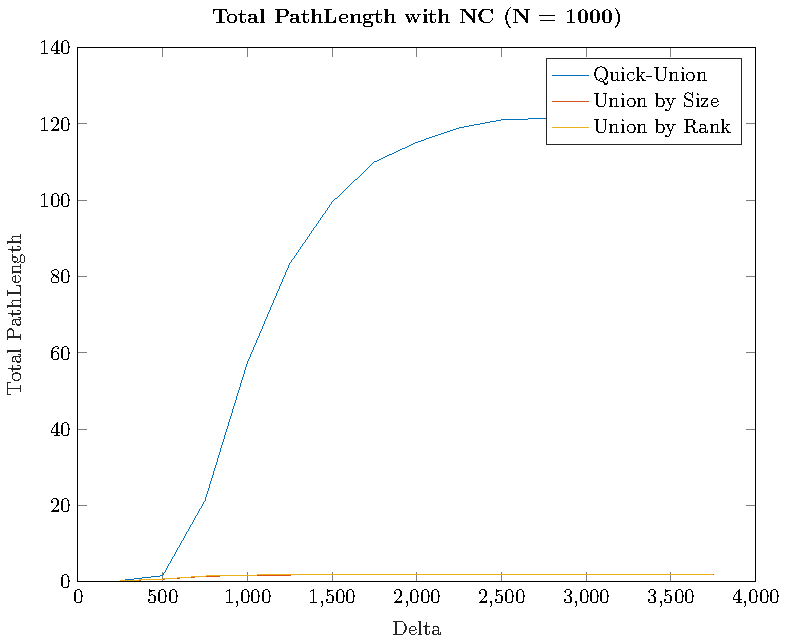
\includegraphics[width=\textwidth]{../images/plotNCFull1000_PathLength.pdf}
        \caption{Path Lengths with different union strategies with $n = 1000$}
    \end{subfigure}%
    \hfill
    % Subfigure 2
    \begin{subfigure}{0.32\textwidth}
        \centering
        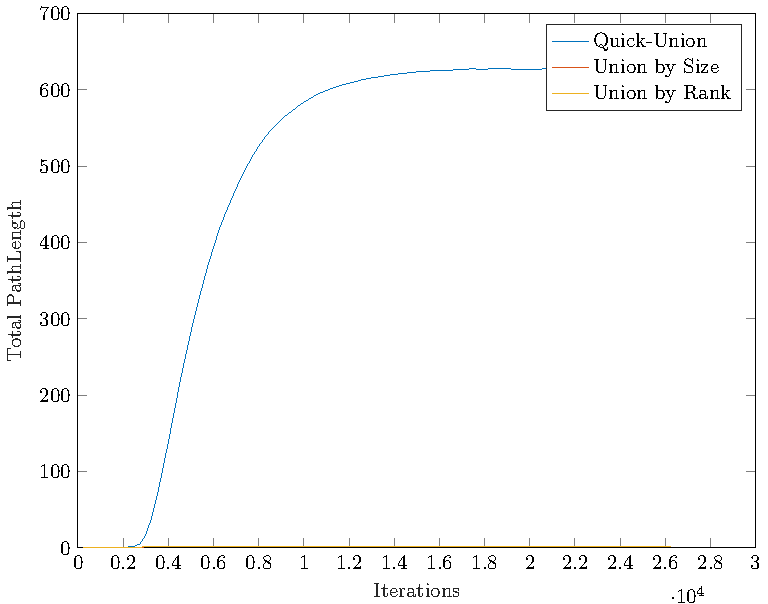
\includegraphics[width=\textwidth]{../images/plotNCFull5000_PathLength.pdf}
        \caption{Path Lengths with different union strategies with $n = 5000$}
    \end{subfigure}%
    \hfill
    % Subfigure 3
    \begin{subfigure}{0.32\textwidth}
        \centering
        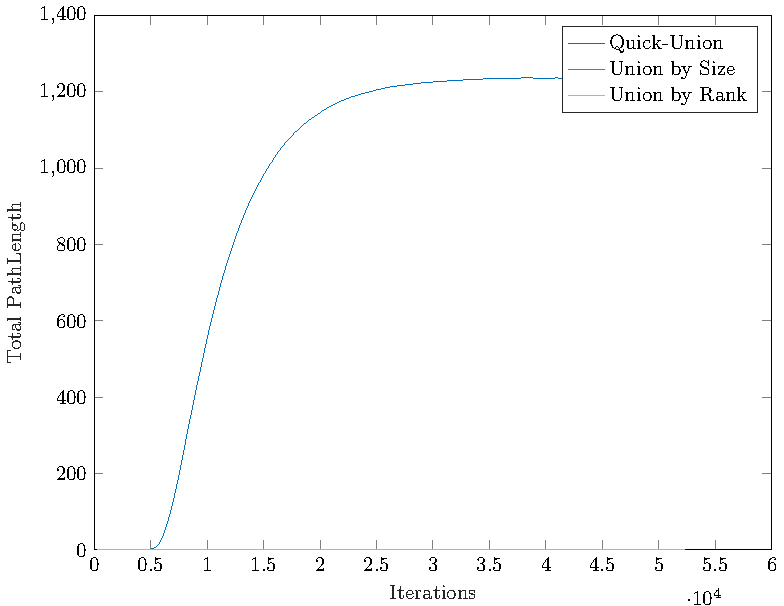
\includegraphics[width=\textwidth]{../images/plotNCFull10000_PathLength.pdf}
        \caption{Path Lengths with different union strategies with $n = 10000$}
    \end{subfigure}

    \caption{Total Path Length normalized with No Compression}
    \label{fig:tplNC}
\end{figure}

\begin{figure}[ht]
    \centering
    % Subfigure 1
    \begin{subfigure}{0.32\textwidth}
        \centering
        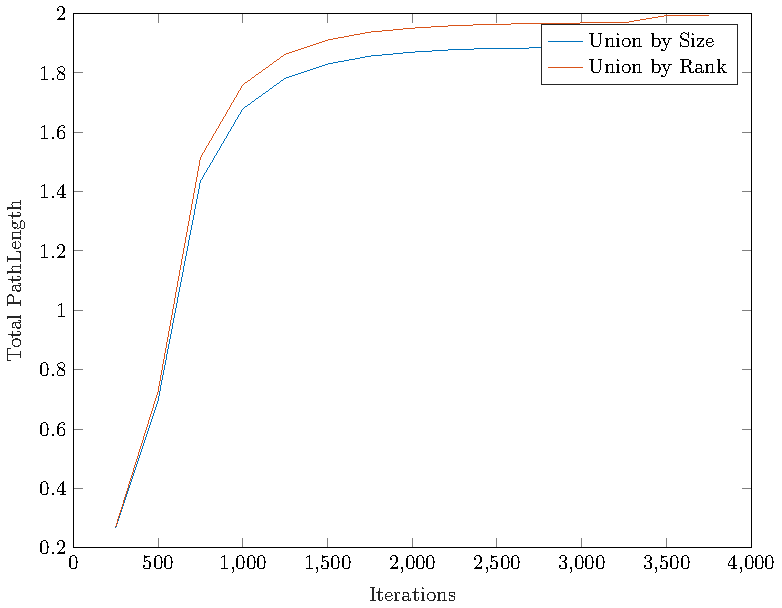
\includegraphics[width=\textwidth]{../images/plotNCNonFull1000_PathLength.pdf}
        \caption{Path Lengths with different union strategies with $n = 1000$}
    \end{subfigure}%
    \hfill
    % Subfigure 2
    \begin{subfigure}{0.32\textwidth}
        \centering
        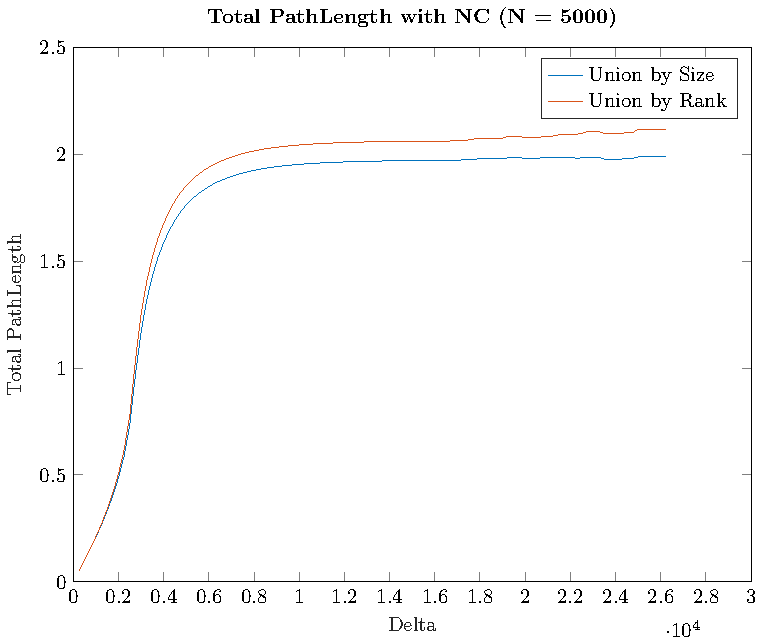
\includegraphics[width=\textwidth]{../images/plotNCNonFull5000_PathLength.pdf}
        \caption{Path Lengths with different union strategies with $n = 5000$}
    \end{subfigure}%
    \hfill
    % Subfigure 3
    \begin{subfigure}{0.32\textwidth}
        \centering
        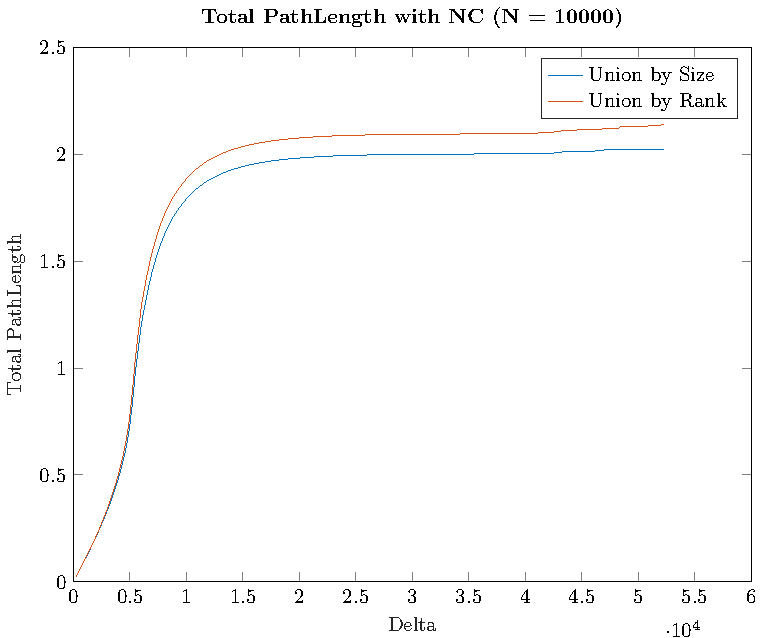
\includegraphics[width=\textwidth]{../images/plotNCNonFull10000_PathLength.pdf}
        \caption{Path Lengths with different union strategies with $n = 10000$}
    \end{subfigure}

    \caption{Total Path Length normalized with No Compression without Quick-Union}
    \label{fig:tplNCNoQU}
\end{figure}


Taking a close look, when you perform a union without compression, the length you add is proportional to the expected length, \(O(\log n)\) because of randomness, which explains why it starts flat and increases quickly. However, as you continue performing more unions, the probability that the pair is already connected increases, so the union does nothing and the TPL does not change. That is why the shape of both figures seems logarithmic.

\subsubsection{Path Strategy: using Heuristics}

Here we are going to consider the following heuristics for path compression:

\begin{itemize}
    \item The \textbf{Full Compression} heuristic ensures that every element in the path from \( i \) to the representative of the class \( r_i \) will point directly to \( r_i \) by traversing the path twice (first to identify \( r_i \) and second to rearrange the pointers). At the cost of traversing this path twice, we expect to speed up future find operations involving a class where this heuristic has been applied. 
    \item Traversing a path twice might not always be the best option so, in order to speed up future find operations, we are going to decrement path lengths within the class by making that every node points to its grandparent as long as this exists. That is what \textbf{Path Splitting} and \textbf{Path Halving} does. The only difference between Path Splitting and Halving is that in splitting we will always make every node point to its grandparent (as long as they exists) while in halving we are going to do that operation every other node (so we expect to end sooner a find operation).
\end{itemize}


As expected, Figure \ref{fig:tplH} clearly shows that Quick-Union starts increasing its TPL faster than the other methods. There is a considerable initial increment, but it quickly starts decreasing, which aligns with expectations—the more find operations we perform, the more balanced each tree becomes. However, we do not observe a \textit{smooth} decrease in the shape, rather than other union heuristics (see Figure \ref{fig:tplNH}). This suggests that, although there is an improvement in TPL as more find operations are executed, the choice of heuristic for the merge strategy also impacts performance (indeed, there is a drastically improvement on the TPL when it starts decreasing because with a Quick-Union strategy there is much more improvement left to do). Both heuristics Union by Weight and Rank behave in the same way (as we try to not unbalance the trees there is not a noticeable improvement, it reaches stability \textit{soon}).

\begin{figure}[ht]
    \centering
    \begin{subfigure}{0.32\textwidth}
        \centering
        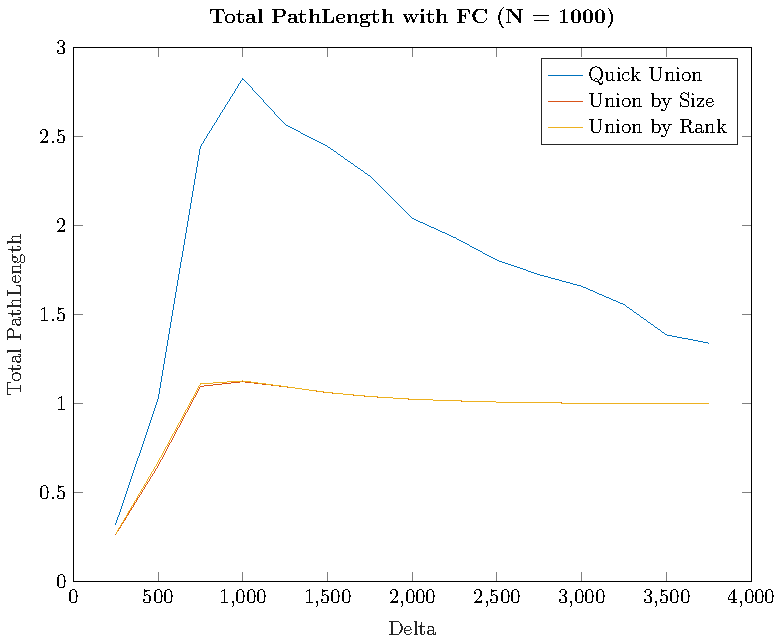
\includegraphics[width=\textwidth]{../images/plotFCFull1000_PathLength.pdf}
        \caption{Path Lengths with different union strategies with $n = 1000$ using Full Compression}
    \end{subfigure}%
    \hfill
    % Subfigure 2
    \begin{subfigure}{0.32\textwidth}
        \centering
        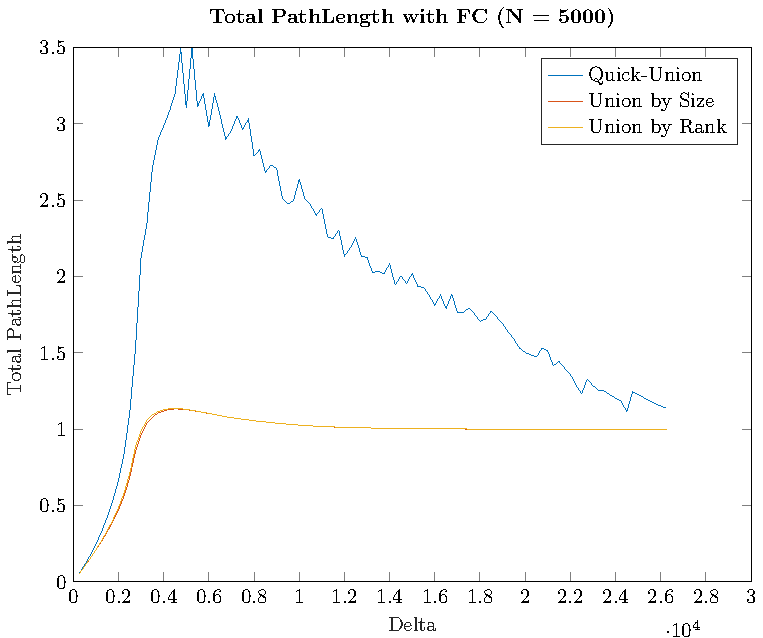
\includegraphics[width=\textwidth]{../images/plotFCFull5000_PathLength.pdf}
        \caption{Path Lengths with different union strategies with $n = 5000$ using Full Compression}
    \end{subfigure}%
    \hfill
    % Subfigure 3
    \begin{subfigure}{0.32\textwidth}
        \centering
        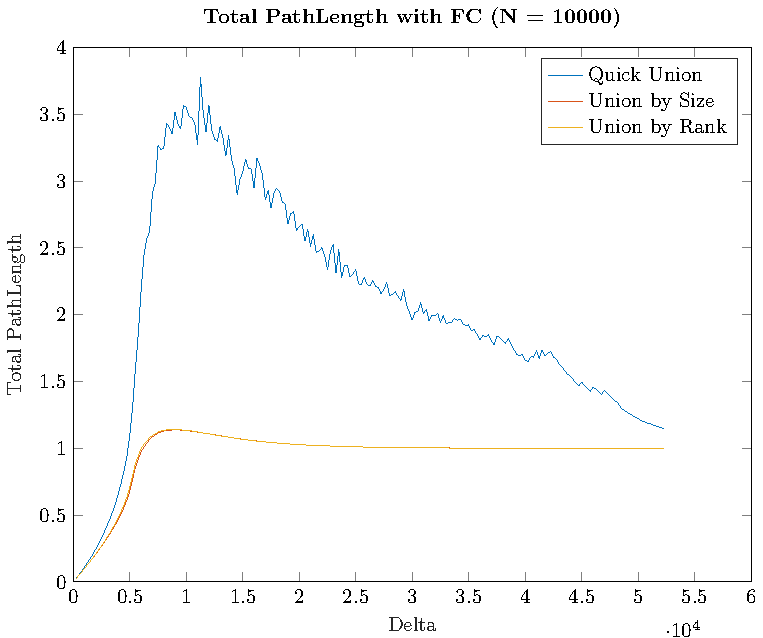
\includegraphics[width=\textwidth]{../images/plotFCFull10000_PathLength.pdf}
        \caption{Path Lengths with different union strategies with $n = 10000$ using Full Compression}
    \end{subfigure}
    % Subfigure 1
    \begin{subfigure}{0.32\textwidth}
        \centering
        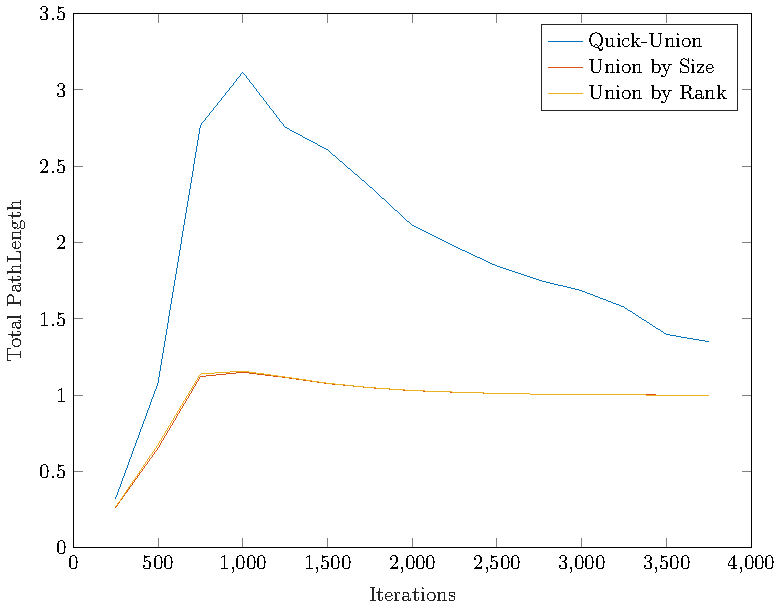
\includegraphics[width=\textwidth]{../images/plotPSFull1000_PathLength.pdf}
        \caption{Path Lengths with different union strategies with $n = 1000$ using Path Splitting}
    \end{subfigure}%
    \hfill
    % Subfigure 2
    \begin{subfigure}{0.32\textwidth}
        \centering
        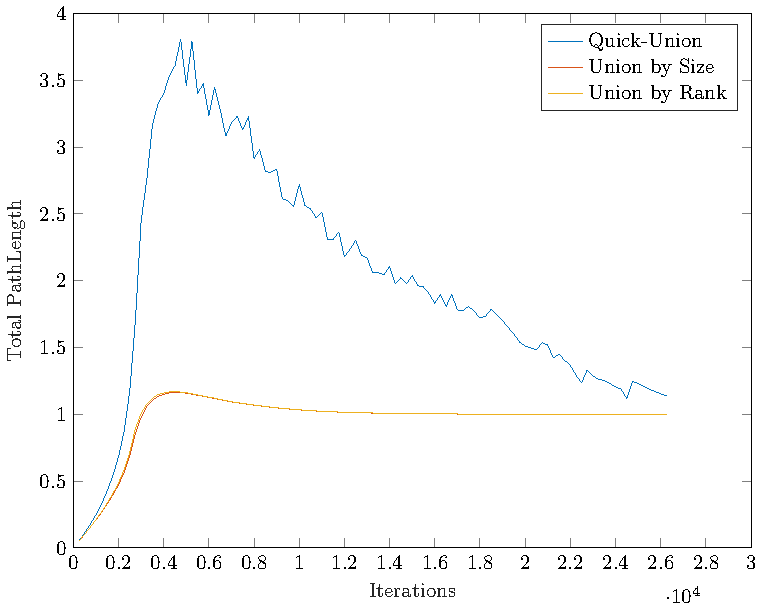
\includegraphics[width=\textwidth]{../images/plotPSFull5000_PathLength.pdf}
        \caption{Path Lengths with different union strategies with $n = 5000$ using Path Splitting}
    \end{subfigure}%
    \hfill
    % Subfigure 3
    \begin{subfigure}{0.32\textwidth}
        \centering
        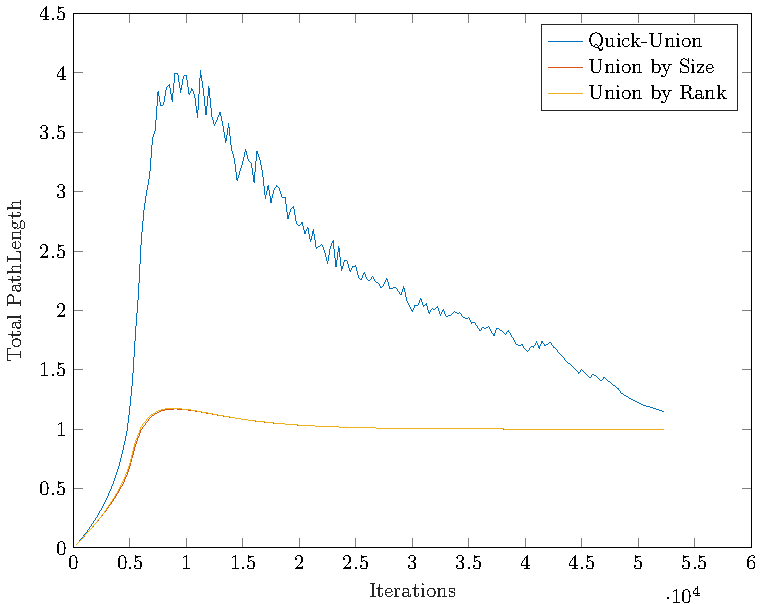
\includegraphics[width=\textwidth]{../images/plotPSFull10000_PathLength.pdf}
        \caption{Path Lengths with different union strategies with $n = 10000$ using Path Splitting}
    \end{subfigure}

    \begin{subfigure}{0.32\textwidth}
        \centering
        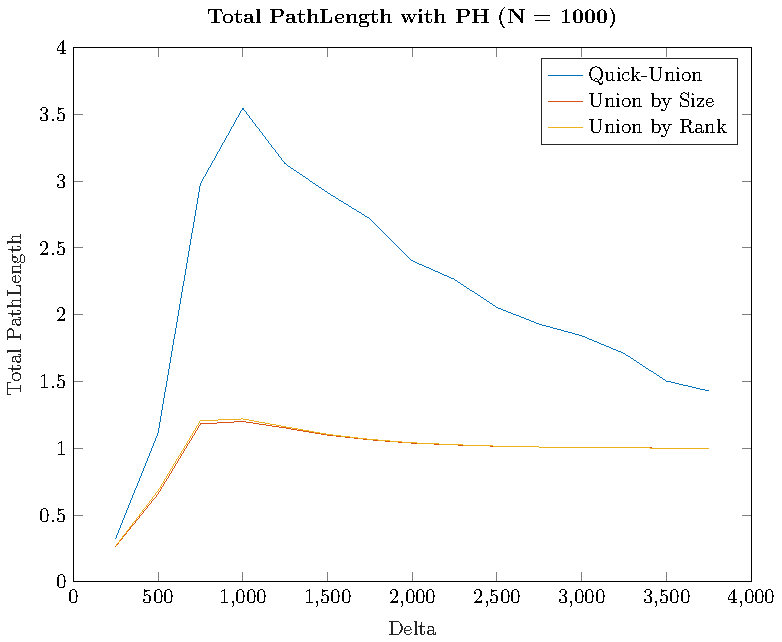
\includegraphics[width=\textwidth]{../images/plotPHFull1000_PathLength.pdf}
        \caption{Path Lengths with different union strategies with $n = 1000$ using Path Halving}
    \end{subfigure}%
    \hfill
    % Subfigure 2
    \begin{subfigure}{0.32\textwidth}
        \centering
        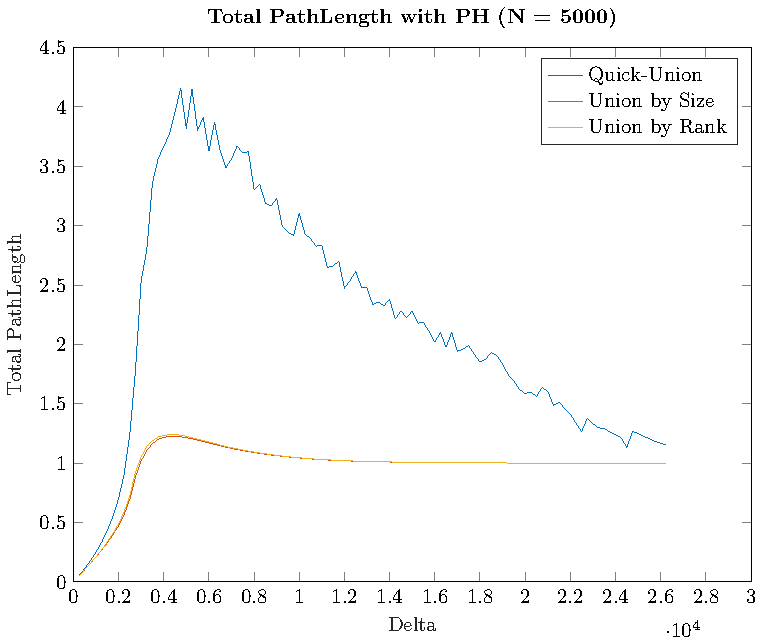
\includegraphics[width=\textwidth]{../images/plotPHFull5000_PathLength.pdf}
        \caption{Path Lengths with different union strategies with $n = 5000$ using Path Halving}
    \end{subfigure}%
    \hfill
    % Subfigure 3
    \begin{subfigure}{0.32\textwidth}
        \centering
        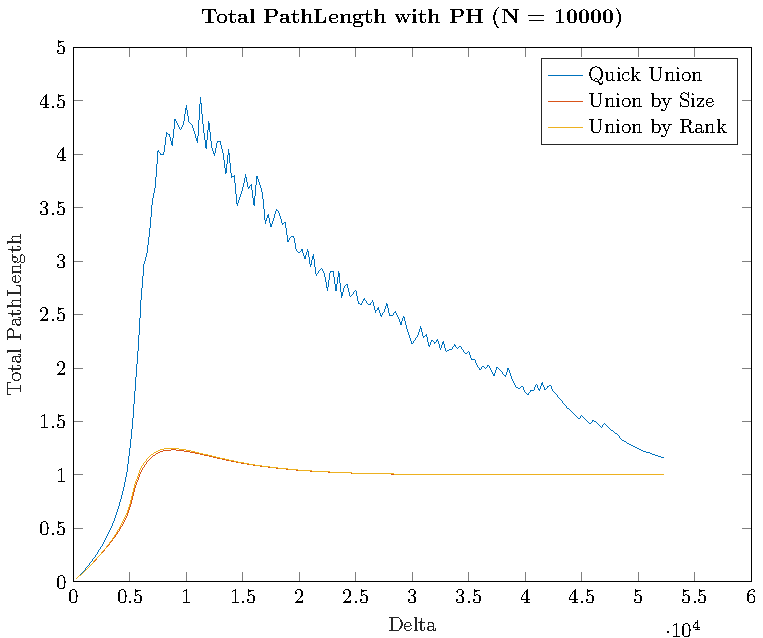
\includegraphics[width=\textwidth]{../images/plotPHFull10000_PathLength.pdf}
        \caption{Path Lengths with different union strategies with $n = 10000$ using Path Halving}
    \end{subfigure}

    \begin{subfigure}{0.32\textwidth}
        \centering
        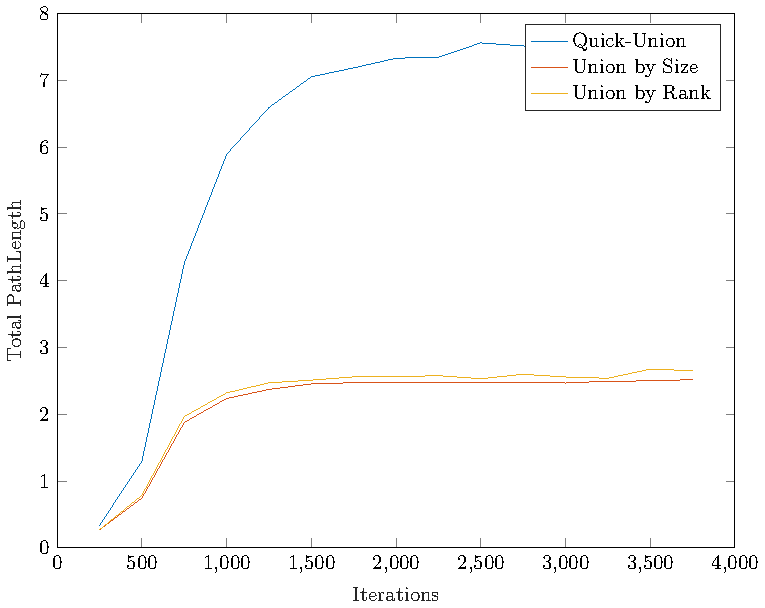
\includegraphics[width=\textwidth]{../images/plotTORFull1000_PathLength.pdf}
        \caption{Path Lengths with different union strategies with $n = 1000$ using Type One Reversal}
    \end{subfigure}%
    \hfill
    % Subfigure 2
    \begin{subfigure}{0.32\textwidth}
        \centering
        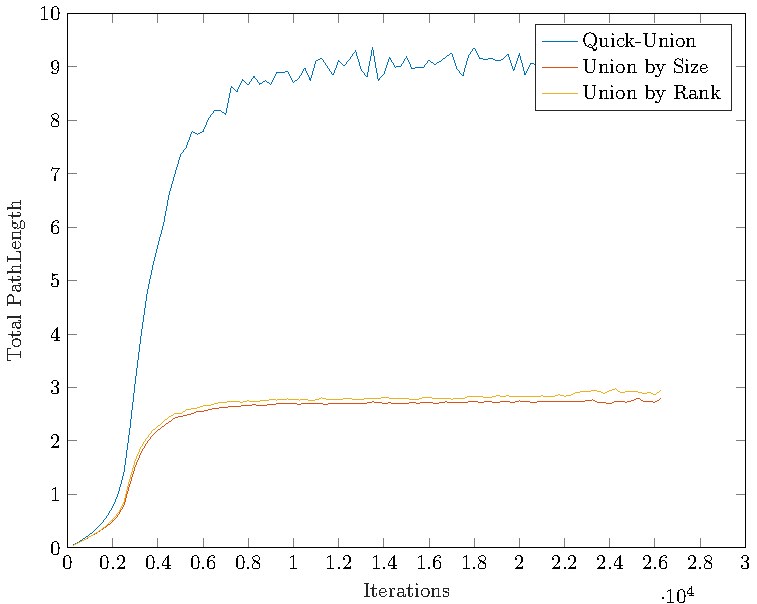
\includegraphics[width=\textwidth]{../images/plotTORFull5000_PathLength.pdf}
        \caption{Path Lengths with different union strategies with $n = 5000$ using Type One Reversal}
    \end{subfigure}%
    \hfill
    % Subfigure 3
    \begin{subfigure}{0.32\textwidth}
        \centering
        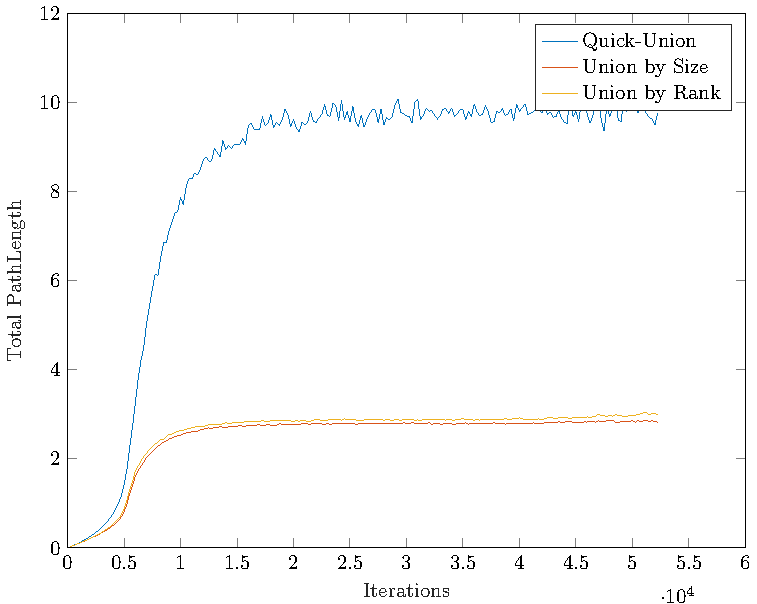
\includegraphics[width=\textwidth]{../images/plotTORFull10000_PathLength.pdf}
        \caption{Path Lengths with different union strategies with $n = 10000$ using Type One Reversal}
    \end{subfigure}

    \caption{Total Path Length normalized for different heuristics}
    \label{fig:tplH}
\end{figure}

\begin{figure}[ht]
    \centering
    \begin{subfigure}{0.32\textwidth}
        \centering
        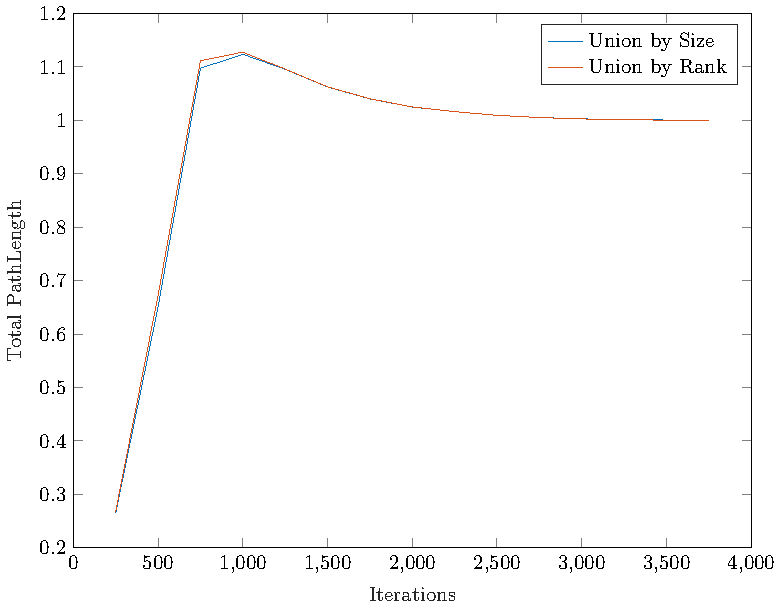
\includegraphics[width=\textwidth]{../images/plotFCNonFull1000_PathLength.pdf}
        \caption{Path Lengths with different union strategies with $n = 1000$ using Full Compression}
    \end{subfigure}%
    \hfill
    % Subfigure 2
    \begin{subfigure}{0.32\textwidth}
        \centering
        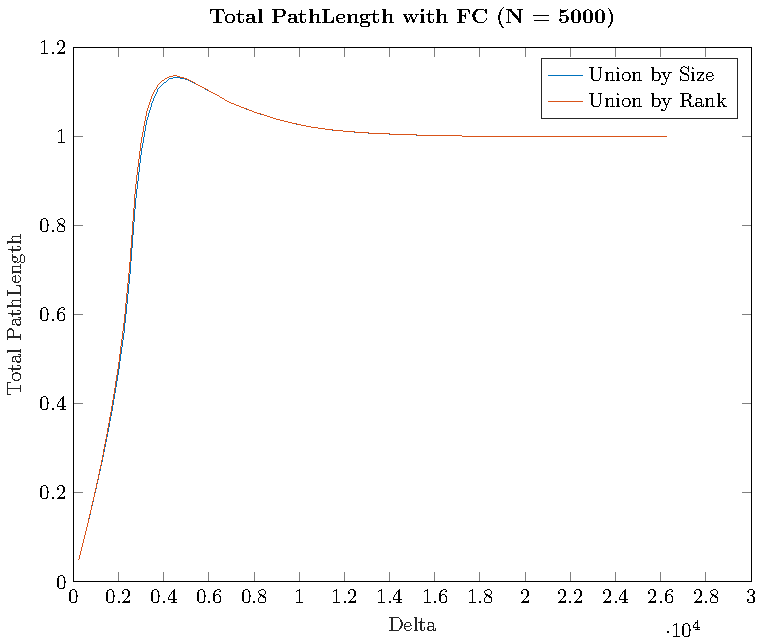
\includegraphics[width=\textwidth]{../images/plotFCNonFull5000_PathLength.pdf}
        \caption{Path Lengths with different union strategies with $n = 5000$ using Full Compression}
    \end{subfigure}%
    \hfill
    % Subfigure 3
    \begin{subfigure}{0.32\textwidth}
        \centering
        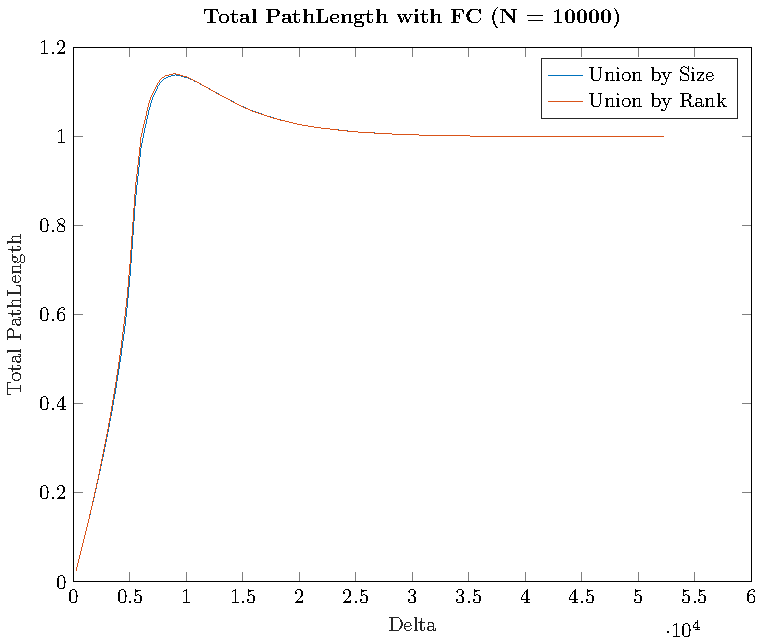
\includegraphics[width=\textwidth]{../images/plotFCNonFull10000_PathLength.pdf}
        \caption{Path Lengths with different union strategies with $n = 10000$ using Full Compression}
    \end{subfigure}
    % Subfigure 1
    \begin{subfigure}{0.32\textwidth}
        \centering
        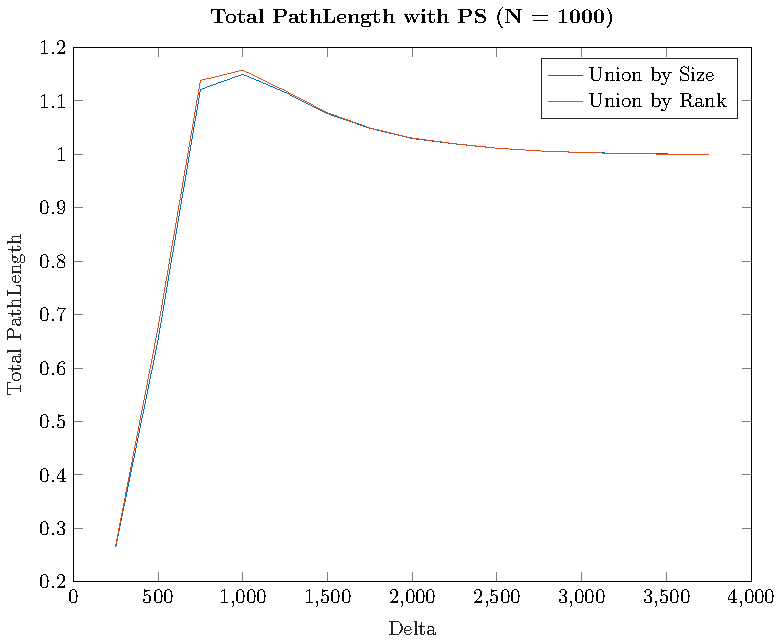
\includegraphics[width=\textwidth]{../images/plotPSNonFull1000_PathLength.pdf}
        \caption{Path Lengths with different union strategies with $n = 1000$ using Path Splitting}
    \end{subfigure}%
    \hfill
    % Subfigure 2
    \begin{subfigure}{0.32\textwidth}
        \centering
        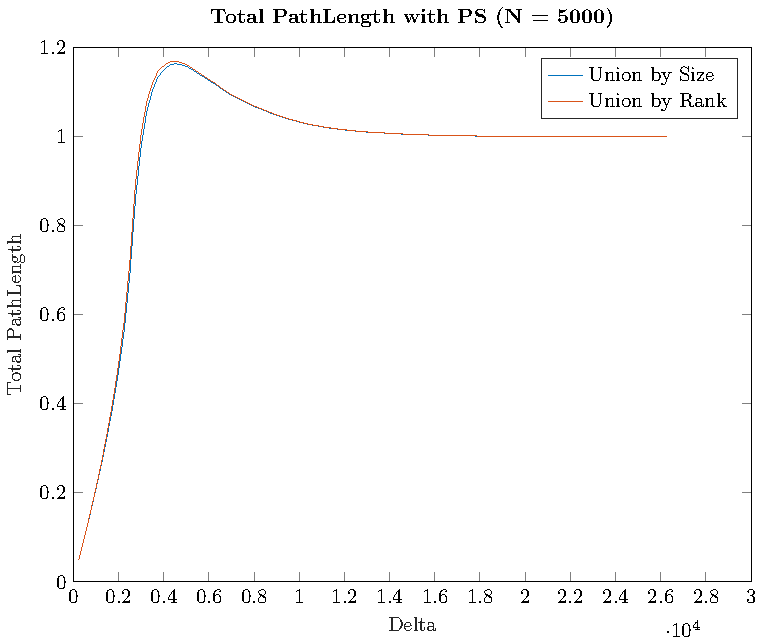
\includegraphics[width=\textwidth]{../images/plotPSNonFull5000_PathLength.pdf}
        \caption{Path Lengths with different union strategies with $n = 5000$ using Path Splitting}
    \end{subfigure}%
    \hfill
    % Subfigure 3
    \begin{subfigure}{0.32\textwidth}
        \centering
        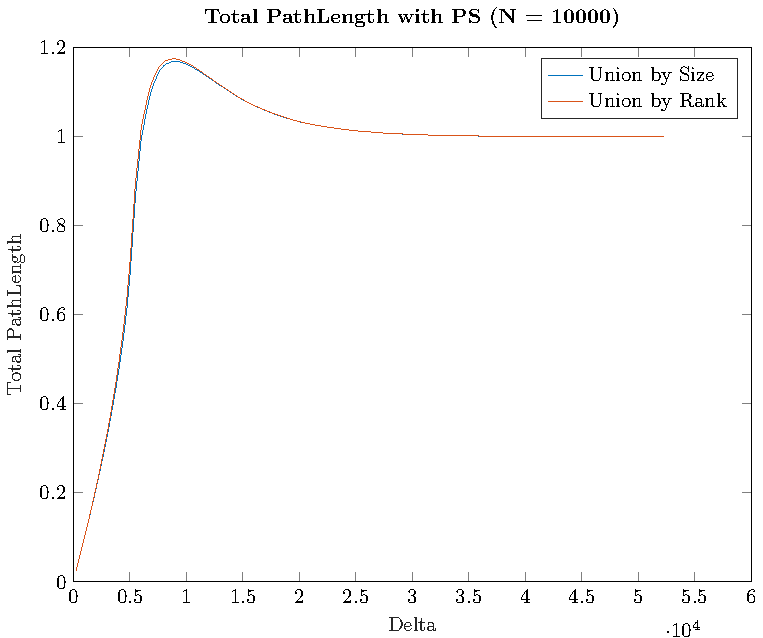
\includegraphics[width=\textwidth]{../images/plotPSNonFull10000_PathLength.pdf}
        \caption{Path Lengths with different union strategies with $n = 10000$ using Path Splitting}
    \end{subfigure}

    \begin{subfigure}{0.32\textwidth}
        \centering
        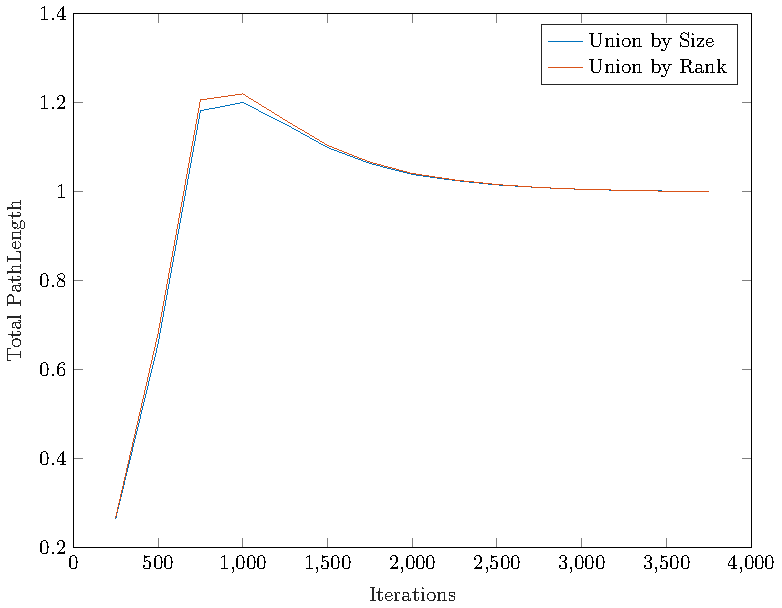
\includegraphics[width=\textwidth]{../images/plotPHNonFull1000_PathLength.pdf}
        \caption{Path Lengths with different union strategies with $n = 1000$ using Path Halving}
    \end{subfigure}%
    \hfill
    % Subfigure 2
    \begin{subfigure}{0.32\textwidth}
        \centering
        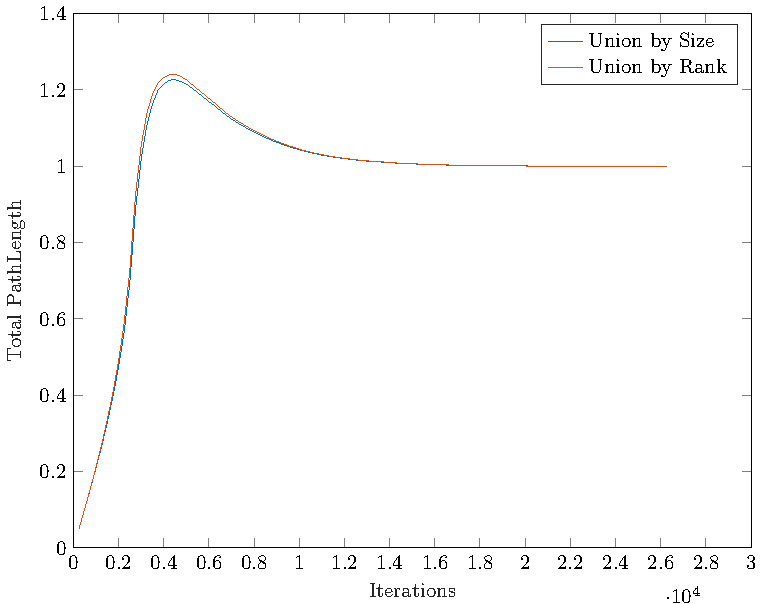
\includegraphics[width=\textwidth]{../images/plotPHNonFull5000_PathLength.pdf}
        \caption{Path Lengths with different union strategies with $n = 5000$ using Path Halving}
    \end{subfigure}%
    \hfill
    % Subfigure 3
    \begin{subfigure}{0.32\textwidth}
        \centering
        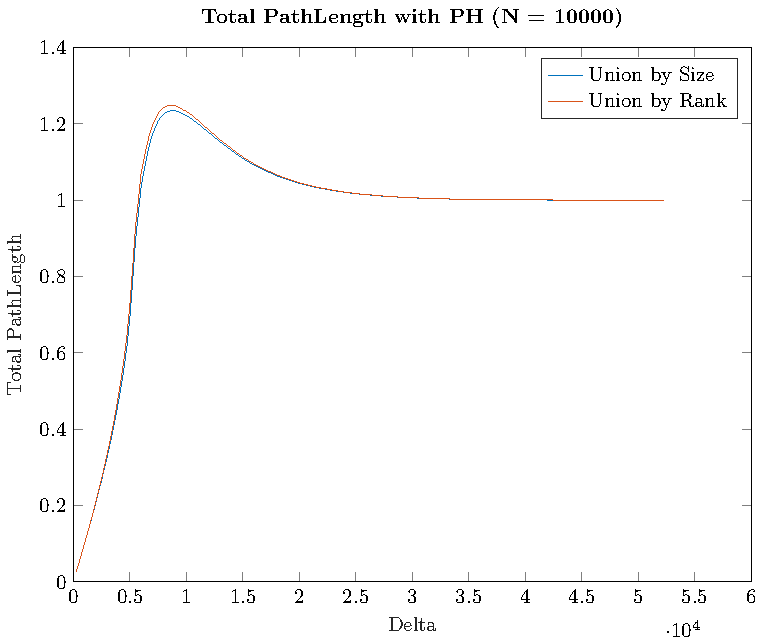
\includegraphics[width=\textwidth]{../images/plotPHNonFull10000_PathLength.pdf}
        \caption{Path Lengths with different union strategies with $n = 10000$ using Path Halving}
    \end{subfigure}
    \begin{subfigure}{0.32\textwidth}
        \centering
        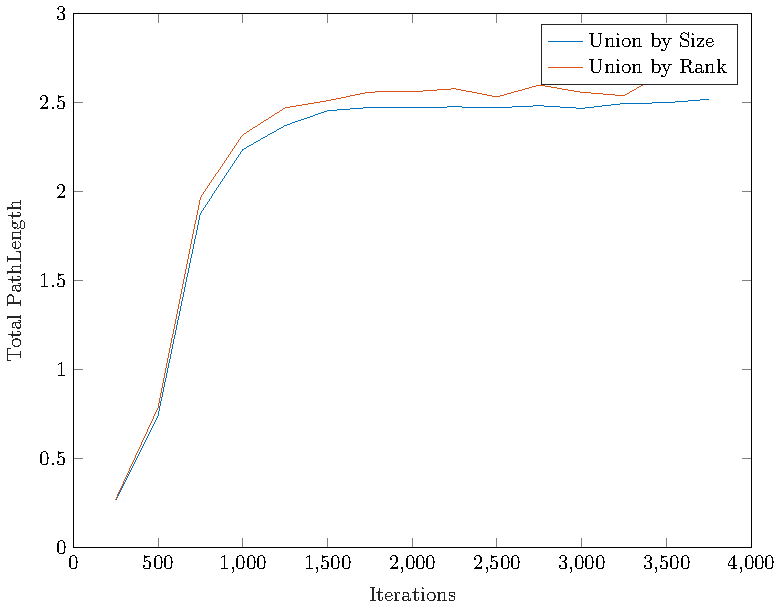
\includegraphics[width=\textwidth]{../images/plotTORNonFull1000_PathLength.pdf}
        \caption{Path Lengths with different union strategies with $n = 1000$ using Type One Reversal}
    \end{subfigure}%
    \hfill
    % Subfigure 2
    \begin{subfigure}{0.32\textwidth}
        \centering
        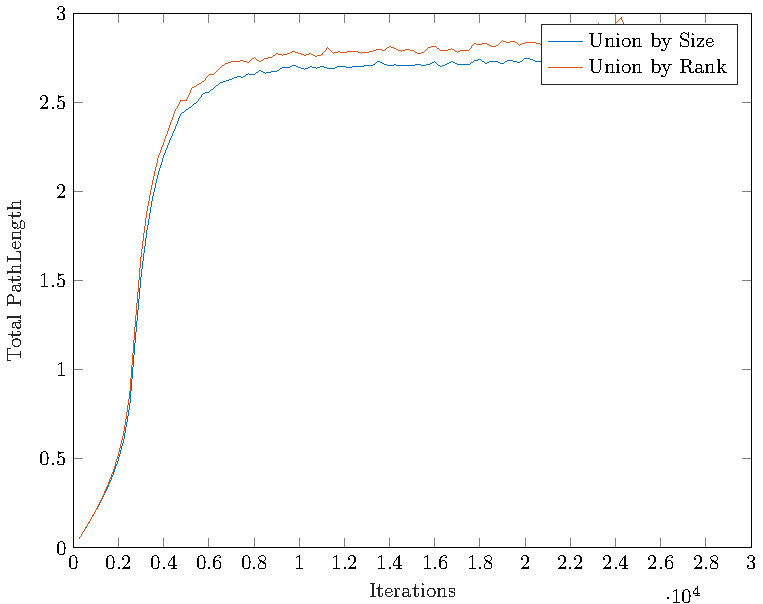
\includegraphics[width=\textwidth]{../images/plotTORNonFull5000_PathLength.pdf}
        \caption{Path Lengths with different union strategies with $n = 5000$ using Type One Reversal}
    \end{subfigure}%
    \hfill
    % Subfigure 3
    \begin{subfigure}{0.32\textwidth}
        \centering
        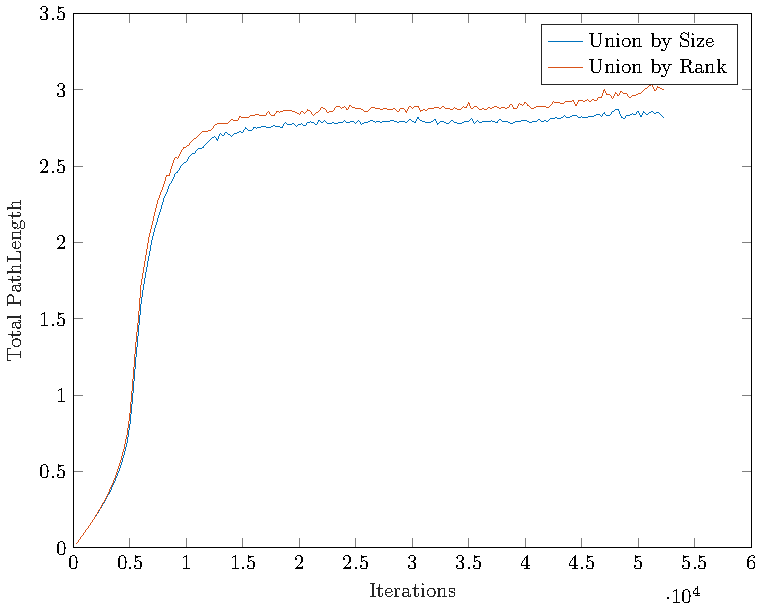
\includegraphics[width=\textwidth]{../images/plotTORNonFull10000_PathLength.pdf}
        \caption{Path Lengths with different union strategies with $n = 10000$ using Type One Reversal}
    \end{subfigure}

    \caption{Total Path Length normalized for different heuristics without Quick-Union}
    \label{fig:tplNH}
\end{figure}


A similar argument can be used to analyze TPUs in Figures \ref{fig:tpuH} and \ref{fig:tpuNH}: because the average TPL in Quick-Union is greater than in Weighted Unions, we traverse more nodes from one element to its representative, resulting in more changes within the path.

A particularly interesting result in Figures \ref{fig:tplNH} and \ref{fig:tpuNH} is that every path compression heuristic with Weighted Unions behaves in exactly the same way. This confirms what Tarjan \& van Leeuwen \cite{tarjan1984worst} proved in their article: every combination of $m$ Union and Find operations on $n$ disjoint sets, using Union by Size/Rank and any of the path compression heuristics (full, splitting, or halving), has a cost of $O(m \cdot \alpha(m,n))$, where $\alpha$ is the inverse Ackermann function. This function is well known for growing extremely slowly—slower even than the iterative logarithm.

\begin{figure}[ht]
    \centering
    \begin{subfigure}{0.32\textwidth}
        \centering
        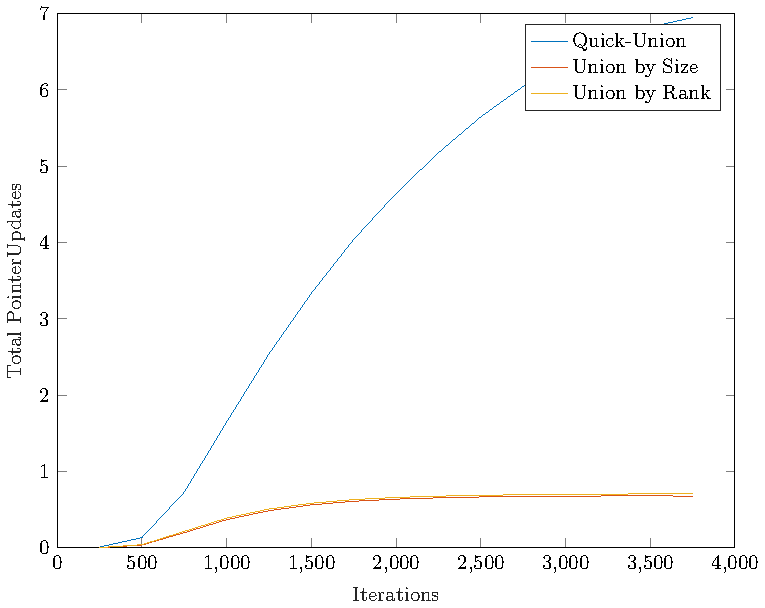
\includegraphics[width=\textwidth]{../images/plotFCFull1000_PointerUpdates.pdf}
        \caption{Pointer Updates with different union strategies with $n = 1000$ using Full Compression}
    \end{subfigure}%
    \hfill
    % Subfigure 2
    \begin{subfigure}{0.32\textwidth}
        \centering
        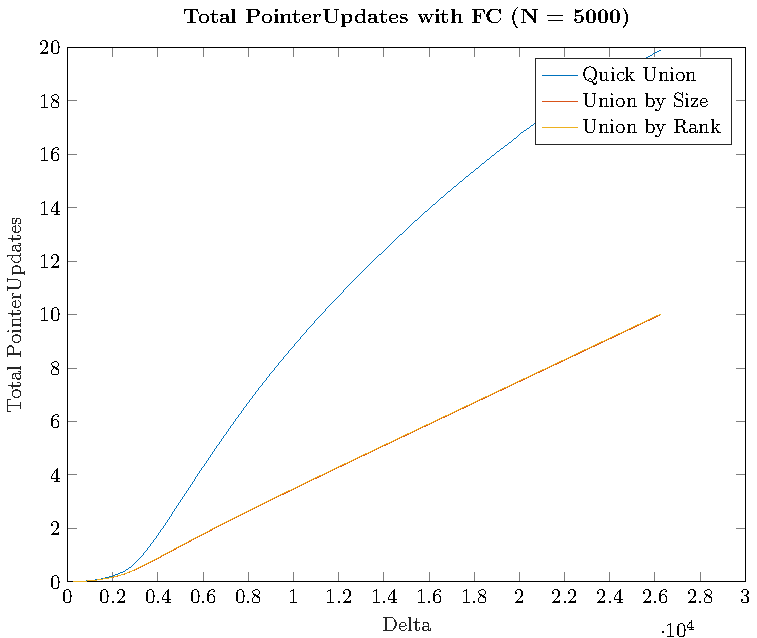
\includegraphics[width=\textwidth]{../images/plotFCFull5000_PointerUpdates.pdf}
        \caption{Pointer Updates with different union strategies with $n = 5000$ using Full Compression}
    \end{subfigure}%
    \hfill
    % Subfigure 3
    \begin{subfigure}{0.32\textwidth}
        \centering
        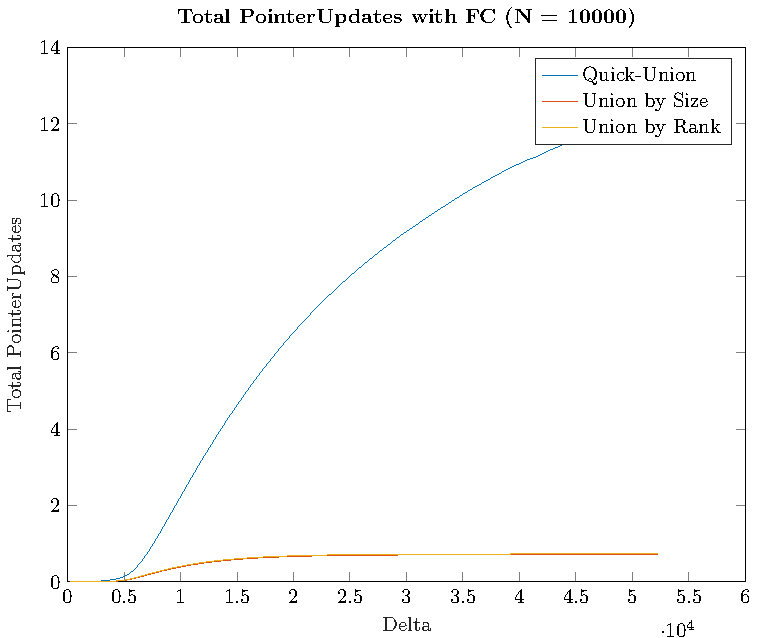
\includegraphics[width=\textwidth]{../images/plotFCFull10000_PointerUpdates.pdf}
        \caption{Pointer Updates with different union strategies with $n = 10000$ using Full Compression}
    \end{subfigure}
    % Subfigure 1
    \begin{subfigure}{0.32\textwidth}
        \centering
        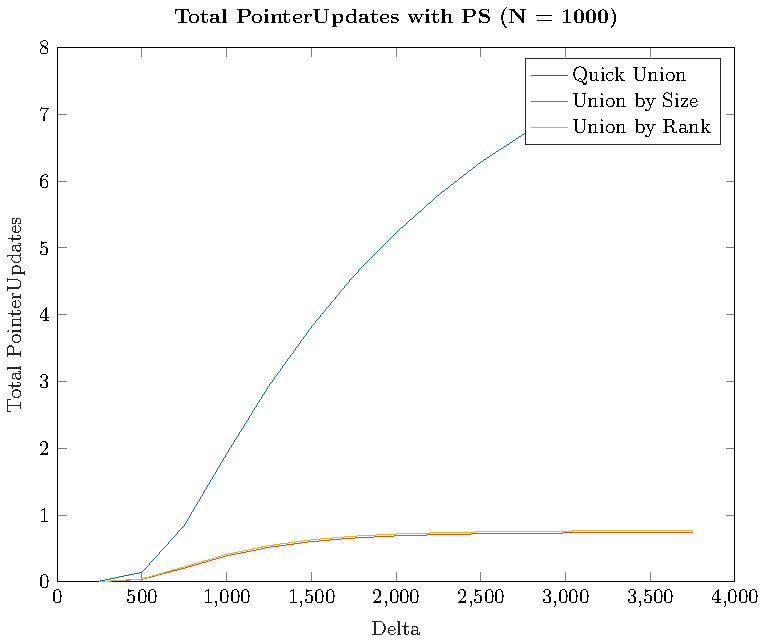
\includegraphics[width=\textwidth]{../images/plotPSFull1000_PointerUpdates.pdf}
        \caption{Pointer Updates with different union strategies with $n = 1000$ using Path Splitting}
    \end{subfigure}%
    \hfill
    % Subfigure 2
    \begin{subfigure}{0.32\textwidth}
        \centering
        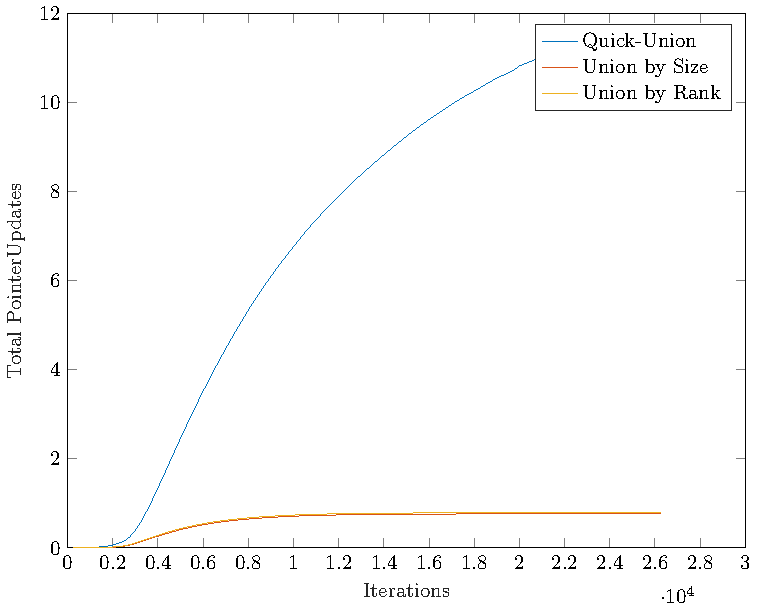
\includegraphics[width=\textwidth]{../images/plotPSFull5000_PointerUpdates.pdf}
        \caption{Pointer Updates with different union strategies with $n = 5000$ using Path Splitting}
    \end{subfigure}%
    \hfill
    % Subfigure 3
    \begin{subfigure}{0.32\textwidth}
        \centering
        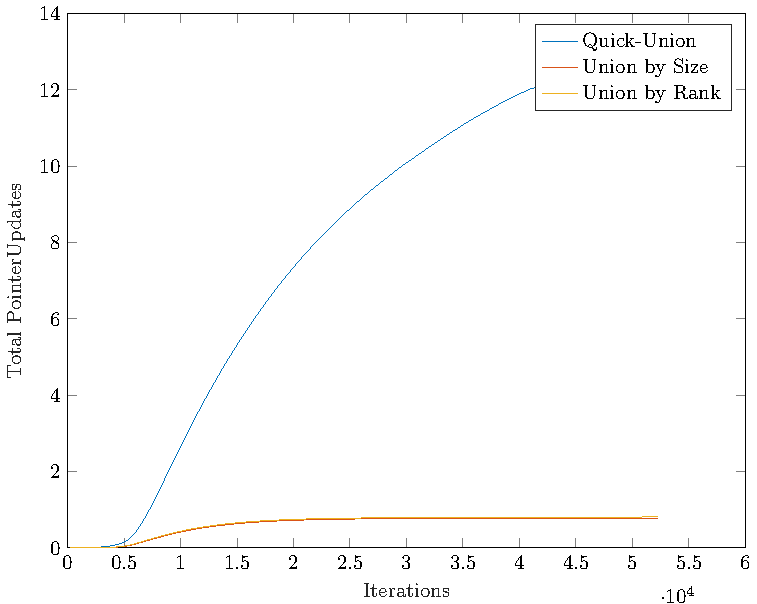
\includegraphics[width=\textwidth]{../images/plotPSFull10000_PointerUpdates.pdf}
        \caption{Pointer Updates with different union strategies with $n = 10000$ using Path Splitting}
    \end{subfigure}

    \begin{subfigure}{0.32\textwidth}
        \centering
        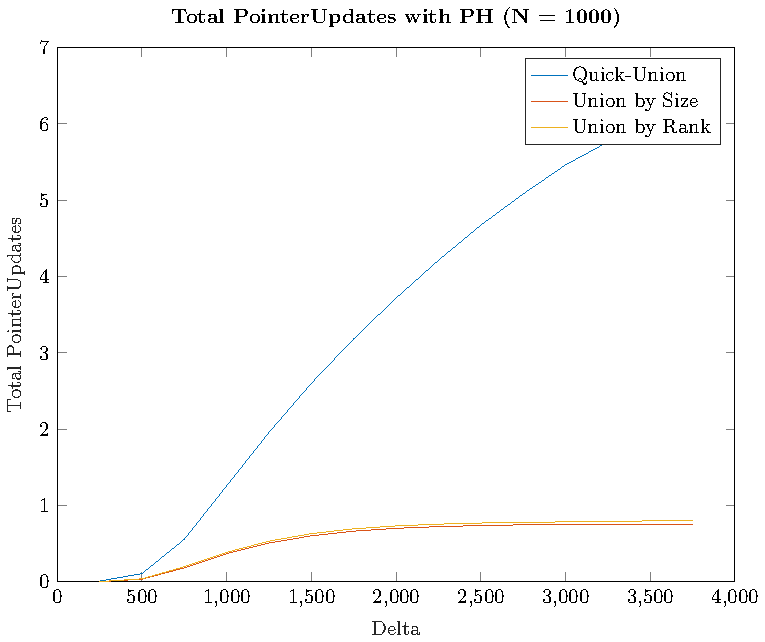
\includegraphics[width=\textwidth]{../images/plotPHFull1000_PointerUpdates.pdf}
        \caption{Pointer Updates with different union strategies with $n = 1000$ using Path Halving}
    \end{subfigure}%
    \hfill
    % Subfigure 2
    \begin{subfigure}{0.32\textwidth}
        \centering
        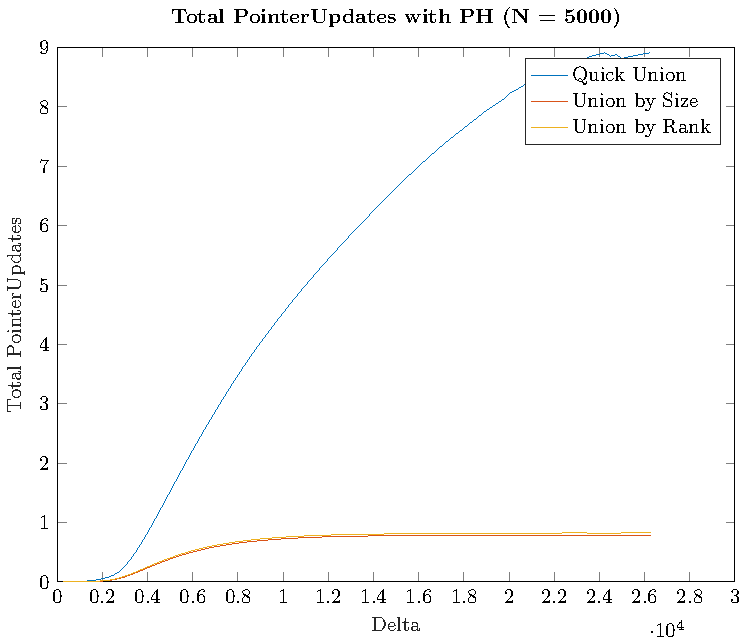
\includegraphics[width=\textwidth]{../images/plotPHFull5000_PointerUpdates.pdf}
        \caption{Pointer Updates with different union strategies with $n = 5000$ using Path Halving}
    \end{subfigure}%
    \hfill
    % Subfigure 3
    \begin{subfigure}{0.32\textwidth}
        \centering
        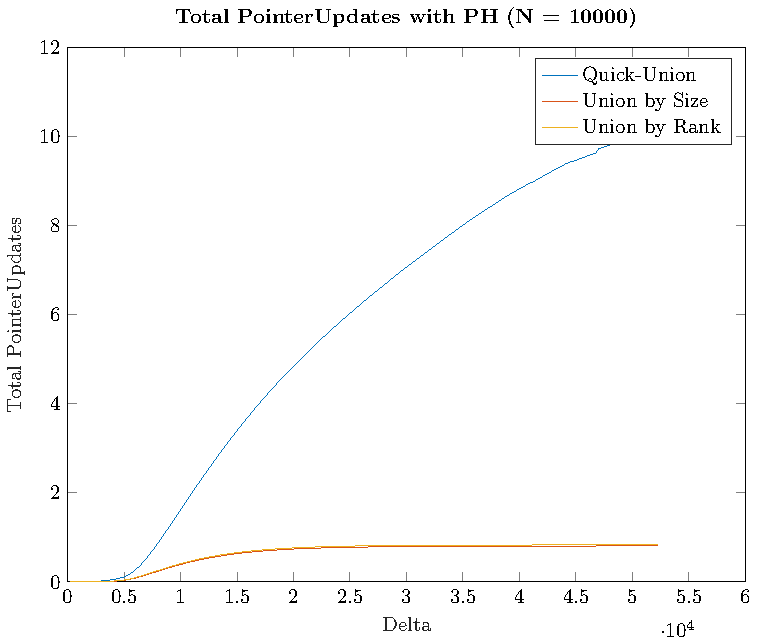
\includegraphics[width=\textwidth]{../images/plotPHFull10000_PointerUpdates.pdf}
        \caption{Pointer Updates with different union strategies with $n = 10000$ using Path Halving}
    \end{subfigure}

    \begin{subfigure}{0.32\textwidth}
        \centering
        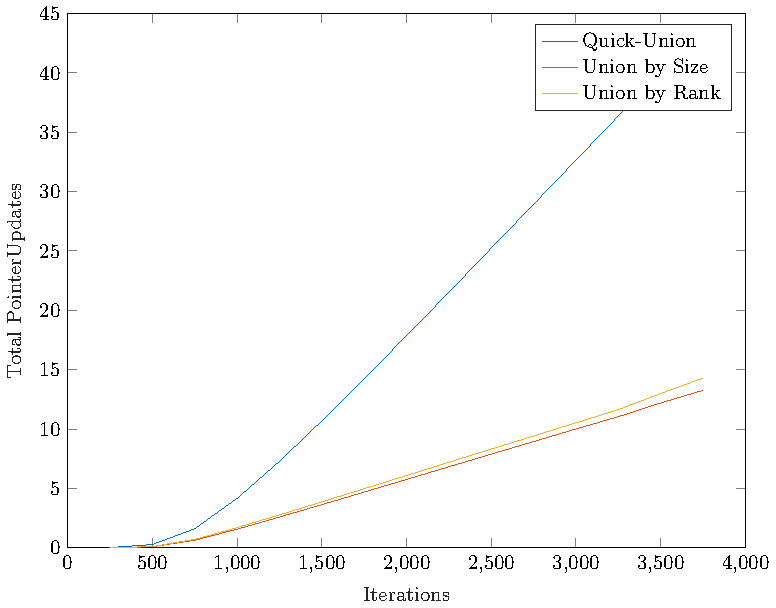
\includegraphics[width=\textwidth]{../images/plotTORFull1000_PointerUpdates.pdf}
        \caption{Pointer Updates with different union strategies with $n = 1000$ using Type One Reversal}
    \end{subfigure}%
    \hfill
    % Subfigure 2
    \begin{subfigure}{0.32\textwidth}
        \centering
        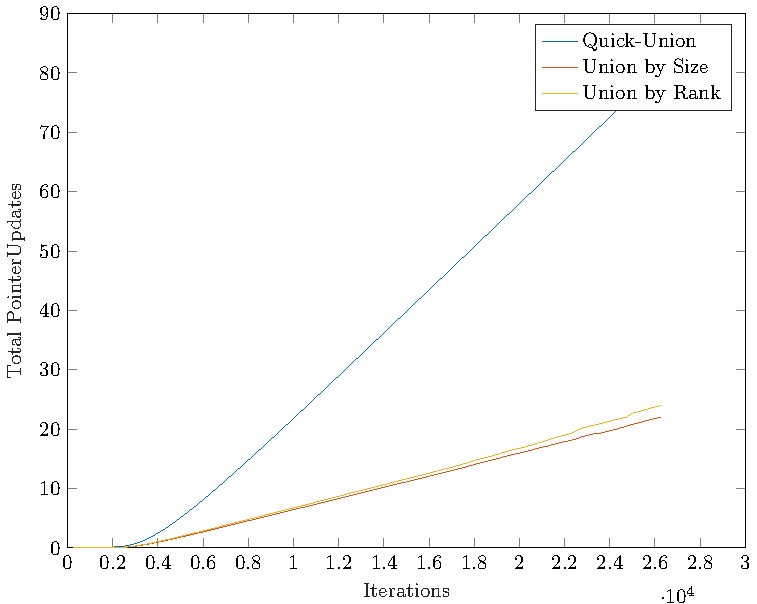
\includegraphics[width=\textwidth]{../images/plotTORFull5000_PointerUpdates.pdf}
        \caption{Pointer Updates with different union strategies with $n = 5000$ using Type One Reversal}
    \end{subfigure}%
    \hfill
    % Subfigure 3
    \begin{subfigure}{0.32\textwidth}
        \centering
        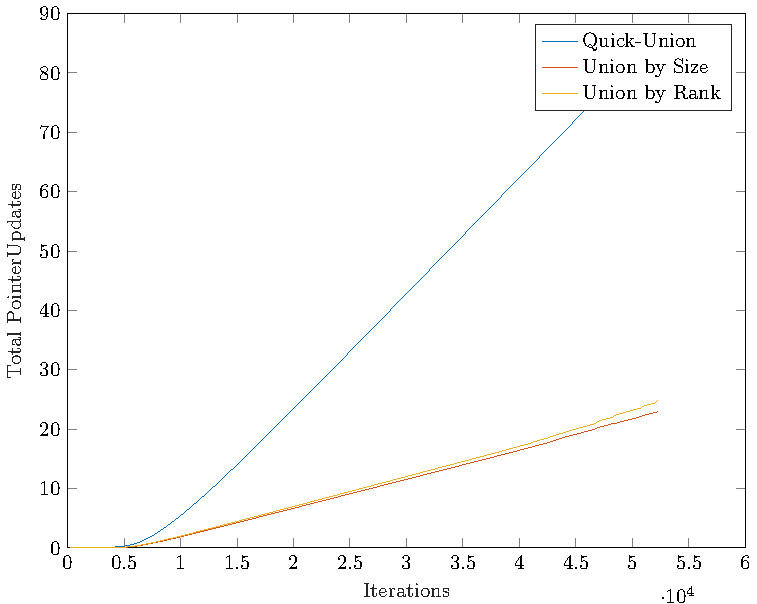
\includegraphics[width=\textwidth]{../images/plotTORFull10000_PointerUpdates.pdf}
        \caption{Pointer Updates with different union strategies with $n = 10000$ using Type One Reversal}
    \end{subfigure}

    \caption{Total Pointer Update normalized using different heuristics}
    \label{fig:tpuH}
\end{figure}


\begin{figure}[ht]
    \centering
    \begin{subfigure}{0.32\textwidth}
        \centering
        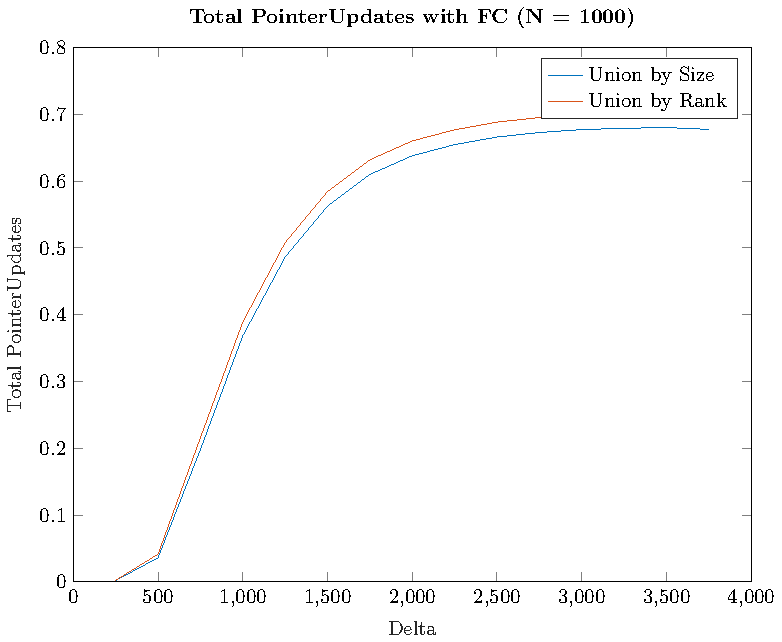
\includegraphics[width=\textwidth]{../images/plotFCNonFull1000_PointerUpdates.pdf}
        \caption{Pointer Updates with different union strategies with $n = 1000$ using Full Compression}
    \end{subfigure}%
    \hfill
    % Subfigure 2
    \begin{subfigure}{0.32\textwidth}
        \centering
        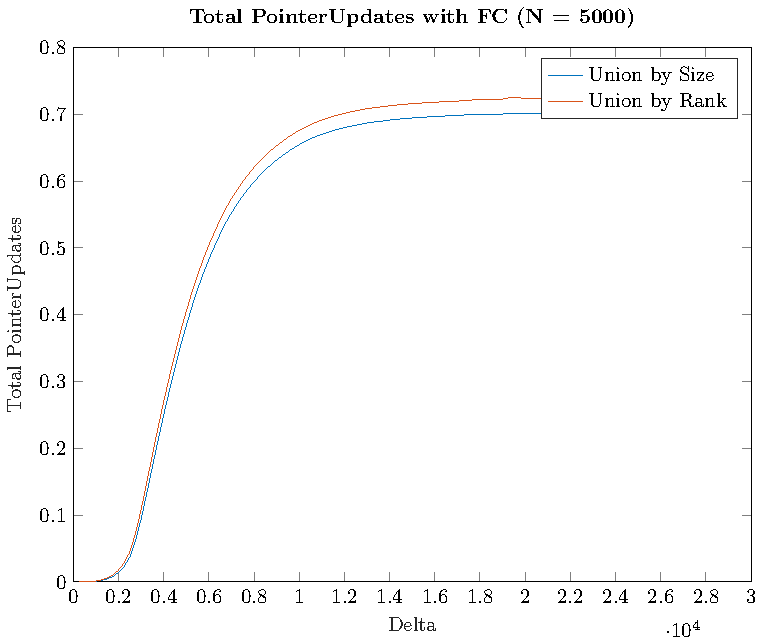
\includegraphics[width=\textwidth]{../images/plotFCNonFull5000_PointerUpdates.pdf}
        \caption{Pointer Updates with different union strategies with $n = 5000$ using Full Compression}
    \end{subfigure}%
    \hfill
    % Subfigure 3
    \begin{subfigure}{0.32\textwidth}
        \centering
        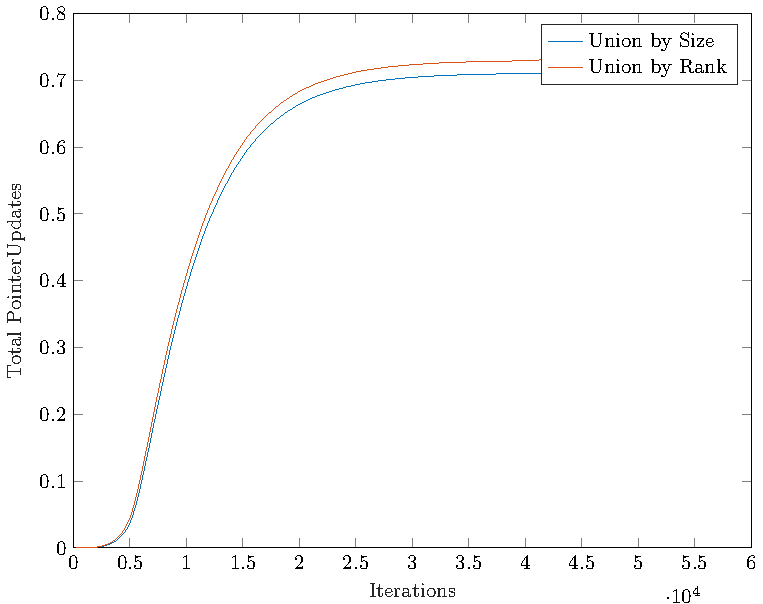
\includegraphics[width=\textwidth]{../images/plotFCNonFull10000_PointerUpdates.pdf}
        \caption{Pointer Updates with different union strategies with $n = 10000$ using Full Compression}
    \end{subfigure}
    % Subfigure 1
    \begin{subfigure}{0.32\textwidth}
        \centering
        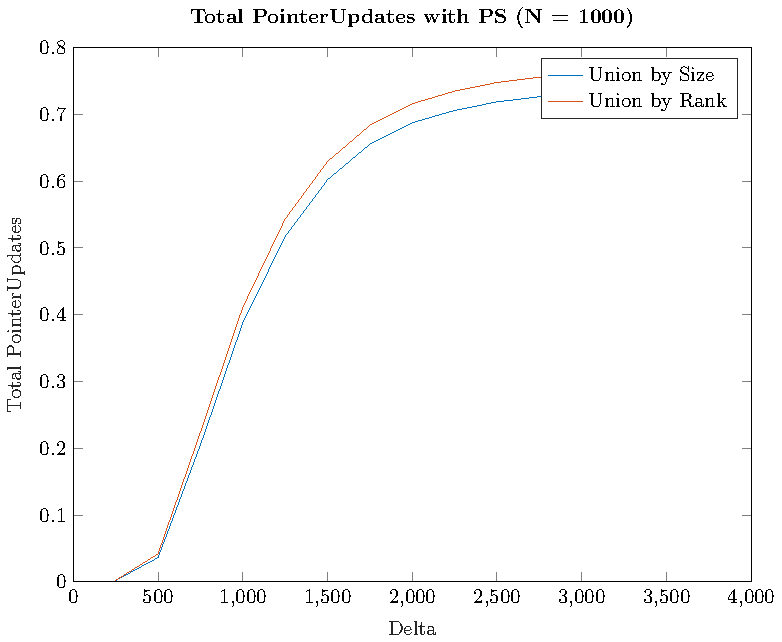
\includegraphics[width=\textwidth]{../images/plotPSNonFull1000_PointerUpdates.pdf}
        \caption{Pointer Updates with different union strategies with $n = 1000$ using Path Splitting}
    \end{subfigure}%
    \hfill
    % Subfigure 2
    \begin{subfigure}{0.32\textwidth}
        \centering
        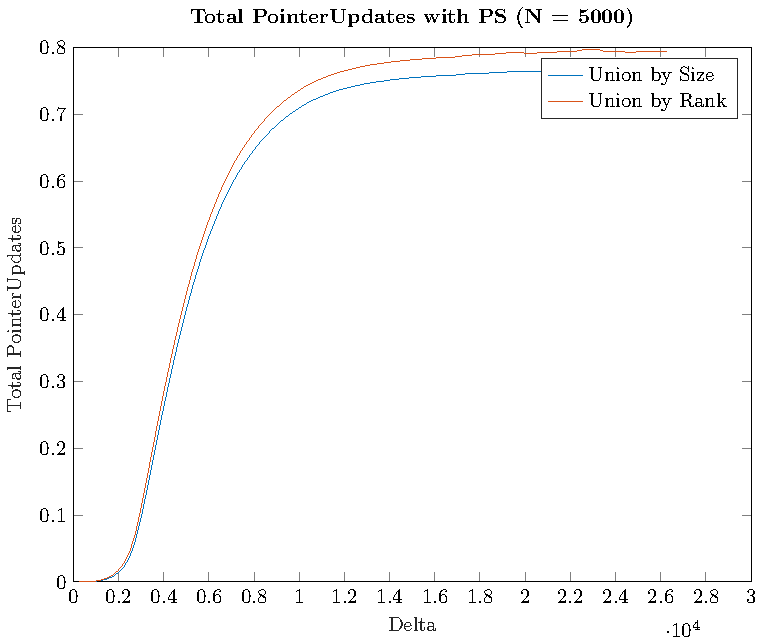
\includegraphics[width=\textwidth]{../images/plotPSNonFull5000_PointerUpdates.pdf}
        \caption{Pointer Updates with different union strategies with $n = 5000$ using Path Splitting}
    \end{subfigure}%
    \hfill
    % Subfigure 3
    \begin{subfigure}{0.32\textwidth}
        \centering
        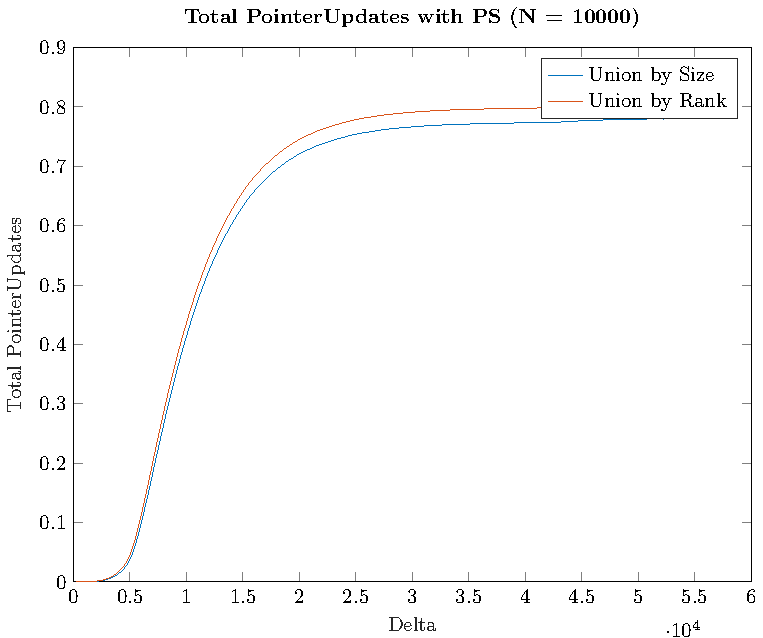
\includegraphics[width=\textwidth]{../images/plotPSNonFull10000_PointerUpdates.pdf}
        \caption{Pointer Updates with different union strategies with $n = 10000$ using Path Splitting}
    \end{subfigure}

    \begin{subfigure}{0.32\textwidth}
        \centering
        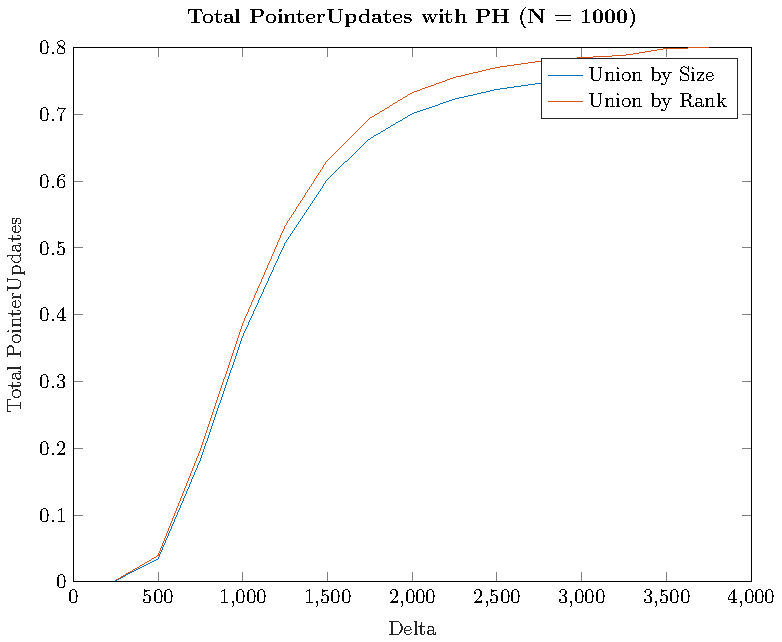
\includegraphics[width=\textwidth]{../images/plotPHNonFull1000_PointerUpdates.pdf}
        \caption{Pointer Updates with different union strategies with $n = 1000$ using Path Halving}
    \end{subfigure}%
    \hfill
    % Subfigure 2
    \begin{subfigure}{0.32\textwidth}
        \centering
        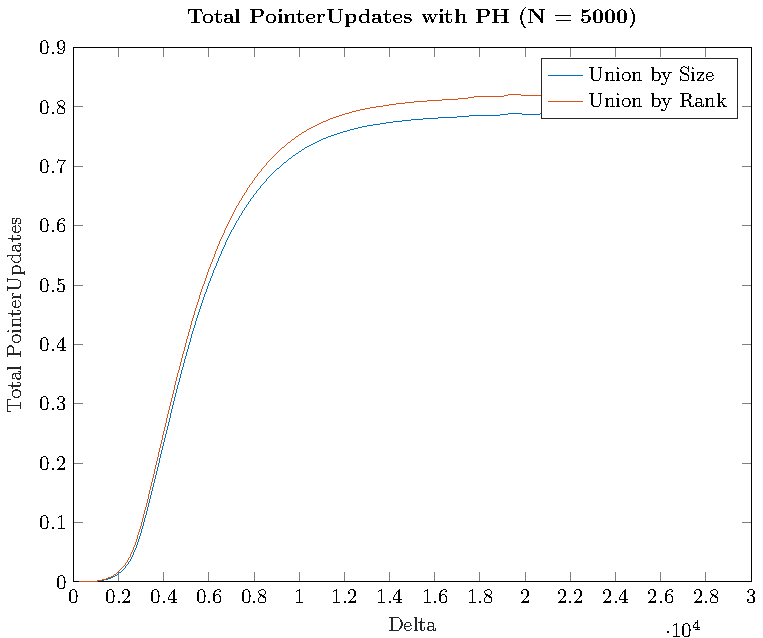
\includegraphics[width=\textwidth]{../images/plotPHNonFull5000_PointerUpdates.pdf}
        \caption{Pointer Updates with different union strategies with $n = 5000$ using Path Halving}
    \end{subfigure}%
    \hfill
    % Subfigure 3
    \begin{subfigure}{0.32\textwidth}
        \centering
        \includegraphics[width=\textwidth]{../images/plotPHNonFull10000_PointerUpdates.pdf}
        \caption{Pointer Updates with different union strategies with $n = 10000$ using Path Halving}
    \end{subfigure}

    \begin{subfigure}{0.32\textwidth}
        \centering
        \includegraphics[width=\textwidth]{../images/plotTORNonFull1000_PointerUpdates.pdf}
        \caption{Pointer Updates with different union strategies with $n = 1000$ using Type One Reversal}
    \end{subfigure}%
    \hfill
    % Subfigure 2
    \begin{subfigure}{0.32\textwidth}
        \centering
        \includegraphics[width=\textwidth]{../images/plotTORNonFull5000_PointerUpdates.pdf}
        \caption{Pointer Updates with different union strategies with $n = 5000$ using Type One Reversal}
    \end{subfigure}%
    \hfill
    % Subfigure 3
    \begin{subfigure}{0.32\textwidth}
        \centering
        \includegraphics[width=\textwidth]{../images/plotTORNonFull10000_PointerUpdates.pdf}
        \caption{Pointer Updates with different union strategies with $n = 10000$ using Type One Reversal}
    \end{subfigure}

    \caption{Total Pointer Update normalized without Quick-Union}
    \label{fig:tpuNH}
\end{figure}


